\documentclass[11pt]{article}
\setlength{\topmargin}{-1.5cm}
\setlength{\textheight}{23cm}
\setlength{\oddsidemargin}{0mm}
\setlength{\evensidemargin}{0mm}
\setlength{\textwidth}{17cm}
\usepackage{graphicx, color}
\usepackage{amsmath, amssymb, amsthm}
\usepackage{enumerate}
\usepackage{hyperref}
\newcommand{\problem}{\medskip \noindent \textbf}

\begin{document}
\noindent {\large  \textbf{Shawn Pan - AM205 Homework 5}} \medskip
Code is attached as separate files.

\problem{Problem 1}

\begin{tabular}{l | l | l | l}
Method & Starting Point & Steps & Final Point\\
\hline
Steepest Descent & (-1, 1) & 2000 & (0.962, 0.926)\\
Steepest Descent & (0, 1) & 2000 & (0.967, 0.934)\\
Steepest Descent & (2, 1) & 980 & (1, 1)\\
Newton & (-1, 1) & 3 & (1, 1)\\
Newton & (0, 1) & 6 & (1, 1)\\
Newton & (2, 1) & 6 & (1, 1)\\
BFGS & (-1, 1) & 124 & (1, 1)\\
BFGS & (0, 1) & 38 & (1, 1)\\
BFGS & (2, 1) & 45 & (1, 1)
\end{tabular}

\begin{figure}[h!]
  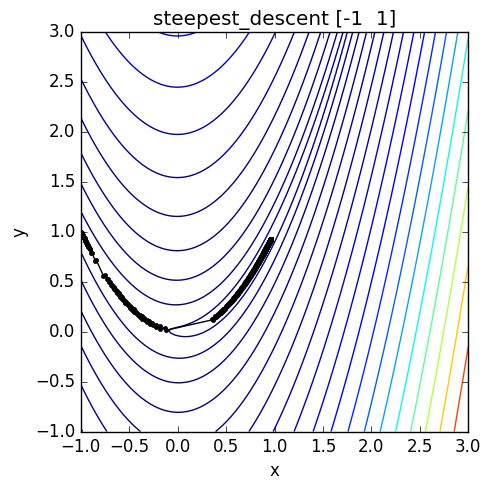
\includegraphics[width=3.3in]{rosenbrock-steepest-descent-1.png}
  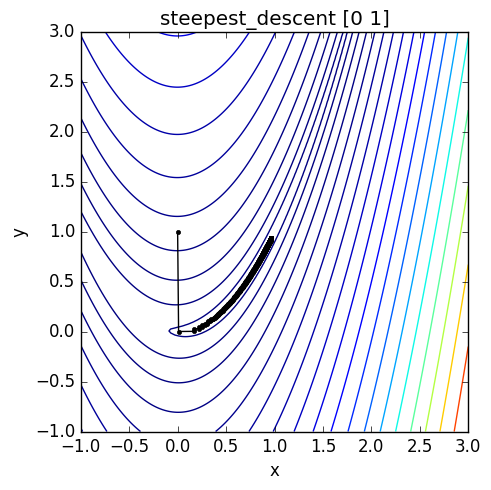
\includegraphics[width=3.3in]{rosenbrock-steepest-descent0.png}
\end{figure}

\pagebreak

\begin{figure}[h!]
  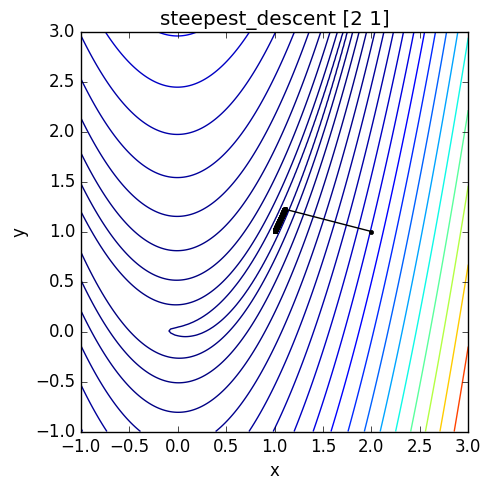
\includegraphics[width=3.3in]{rosenbrock-steepest-descent2.png}
  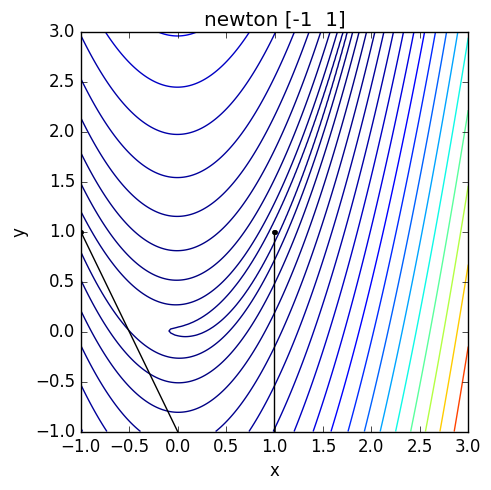
\includegraphics[width=3.3in]{rosenbrock-newton-1.png}
\end{figure}

\begin{figure}[h!]
  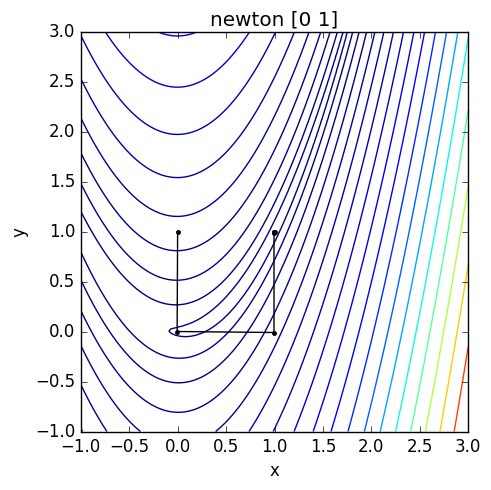
\includegraphics[width=3.3in]{rosenbrock-newton0.png}
  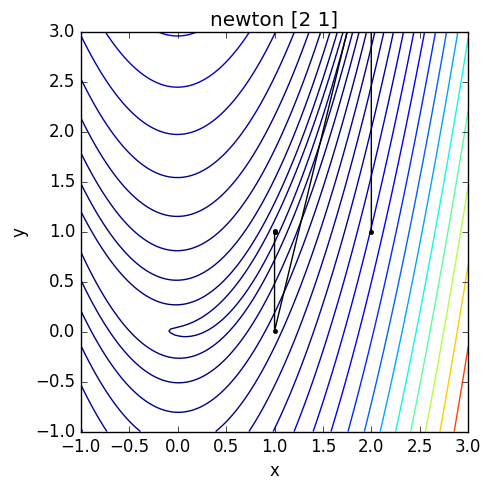
\includegraphics[width=3.3in]{rosenbrock-newton2.png}
\end{figure}

\pagebreak

\begin{figure}[h!]
  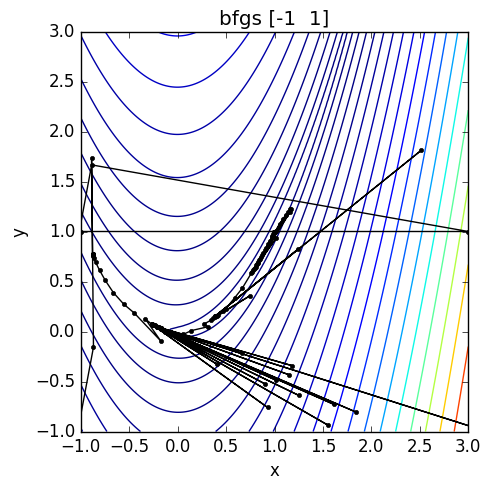
\includegraphics[width=3.3in]{rosenbrock-bfgs-1.png}
  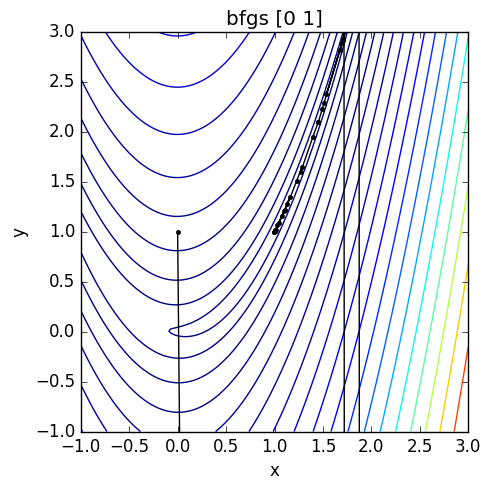
\includegraphics[width=3.3in]{rosenbrock-bfgs0.png}
\end{figure}

\begin{figure}[h!]
  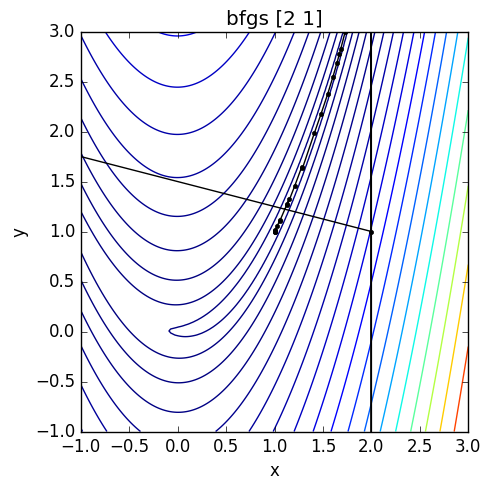
\includegraphics[width=3.3in]{rosenbrock-bfgs2.png}
\end{figure}

\pagebreak

\problem{Problem 2}

\problem{(a)}

Some convenient intermediate terms:
\begin{align*}
\frac{dx}{ds} &= \frac{L}{R} + \sum_{k=1}^{20} \frac{\pi k c_k}{R} \cos \frac{\pi k s}{R}\\
\frac{dy}{ds} &= \sum_{k=1}^{20} \frac{\pi k d_k}{R} \cos \frac{\pi k s}{R}\\
\frac{\partial}{\partial c_i}\frac{dx}{ds} &= \frac{\pi i}{R} \cos \frac{\pi i s}{R}\\
\frac{\partial}{\partial d_i}\frac{dy}{ds} &= \frac{\pi i}{R} \cos \frac{\pi i s}{R}\\
\frac{\partial y}{\partial d_i} &= \sin \frac{\pi i s}{R}\\
A &= \sqrt{\left(\tfrac{dx}{ds}\right)^2 + \left(\tfrac{dy}{ds}\right)^2}
\end{align*}

Gradient components (expressed with intermediate terms above):
\begin{align*}
\frac{\partial r}{\partial c_i} &= \int_0^R \mu (2) \left(A-1\right) \frac{1}{2A} (2) \left(\frac{dx}{ds}\right) \left(\frac{\partial}{\partial c_i}\frac{dx}{ds} \right) ds\\
&= \int_0^R 2 \mu \frac{A - 1}{A} \left(\frac{dx}{ds}\right) \left(\frac{\partial}{\partial c_i}\frac{dx}{ds} \right) ds\\
\frac{\partial r}{\partial d_i} &= \int_0^R \left[ 2 \mu \frac{A - 1}{A} \left(\frac{dy}{ds}\right) \left(\frac{\partial}{\partial d_i}\frac{dy}{ds} \right) - 2 \rho \omega^2 y \left(\frac{\partial y}{\partial d_i}\right) \right] ds
\end{align*}

\problem{(b/c)}

\begin{figure}[h!]
  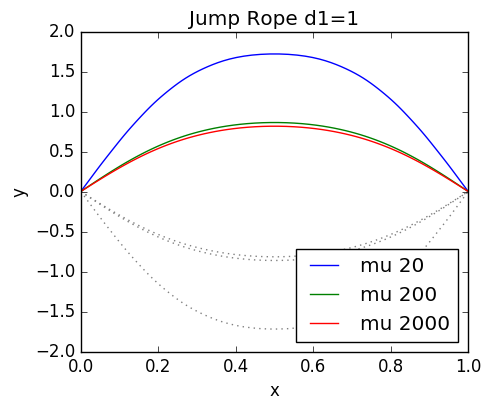
\includegraphics[width=3in]{rope1.png}
  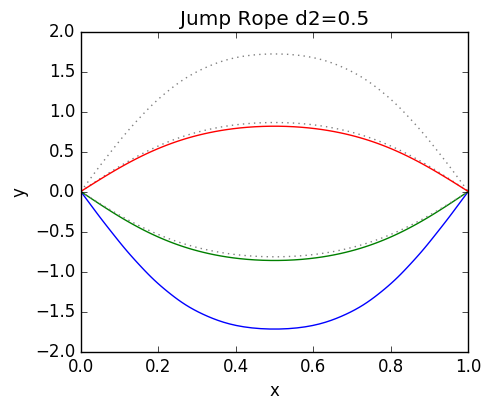
\includegraphics[width=3in]{rope2.png}
\end{figure}

$\mu = 2000$ appears to converge to the same solution, while $\mu = 20$ and $\mu = 200$ appear to converge to alternate solutions reflected across the $x$-axis.  Because all $y$ terms in the residual function are squared, the problem is symmetric and the reflected solutions (shown in grey) have the same energy.

\pagebreak

\problem{Problem 3}

\problem{(a)}

We will the centered finite difference approximation:
$$\frac{\partial^2 \Psi}{\partial x^2} \approx \frac{\Psi(x-h) - 2\Psi(x) + \Psi(x+h)}{h^2}$$

We can express the equation as $H\Psi = E\Psi$, where $H$ is the following matrix with $v_i$ as the potential evaluated on the grid point $i$.
\[
\begin{pmatrix}
\frac{2}{h^2} + v_0 & \frac{-1}{h^2} & 0 & 0 & \dots & 0 & 0\\
\frac{-1}{h^2} &  \frac{2}{h^2} + v_1 & \frac{-1}{h^2} & 0 & \dots & 0 & 0\\
0 & \frac{-1}{h^2} &  \frac{2}{h^2} + v_2 & \frac{-1}{h^2} & \dots & 0 & 0\\
\vdots & \vdots & \vdots & \vdots & \ddots & \vdots & \vdots\\
0 & 0 & 0 & 0 & \dots & \frac{-1}{h^2} & \frac{2}{h^2} + v_{1920}
\end{pmatrix}
\]

Note that truncating the first and last rows is conveniently equavalent to enforcing the zero Dirichlet boundary conditions.  (Technically, this enforces $\Psi(-12-h) = 0$ and $\Psi(12+h) = 0$, but shifting one step doesn't change the numerical result.)

\begin{figure}[h!]
  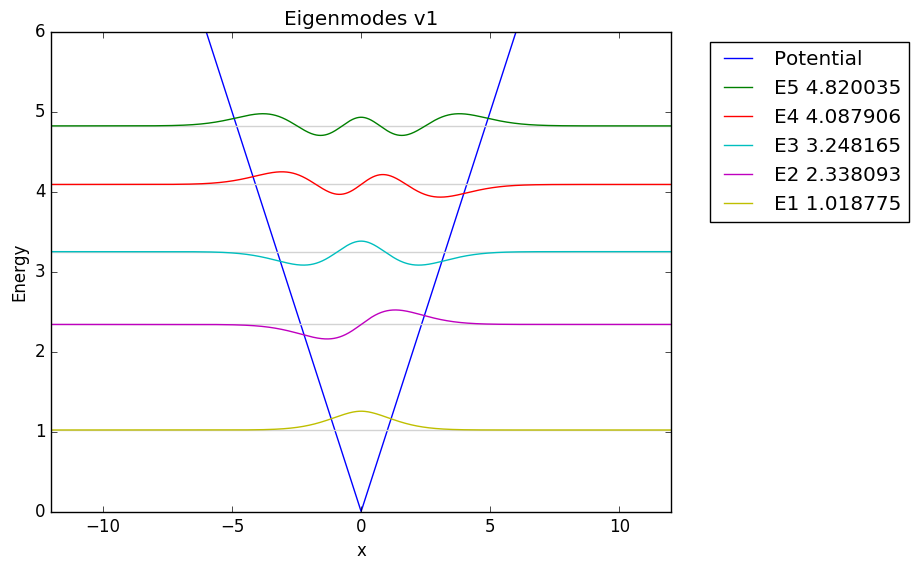
\includegraphics[width=5.5in]{eigv1.png}
\end{figure}

\pagebreak

\begin{figure}[h!]
  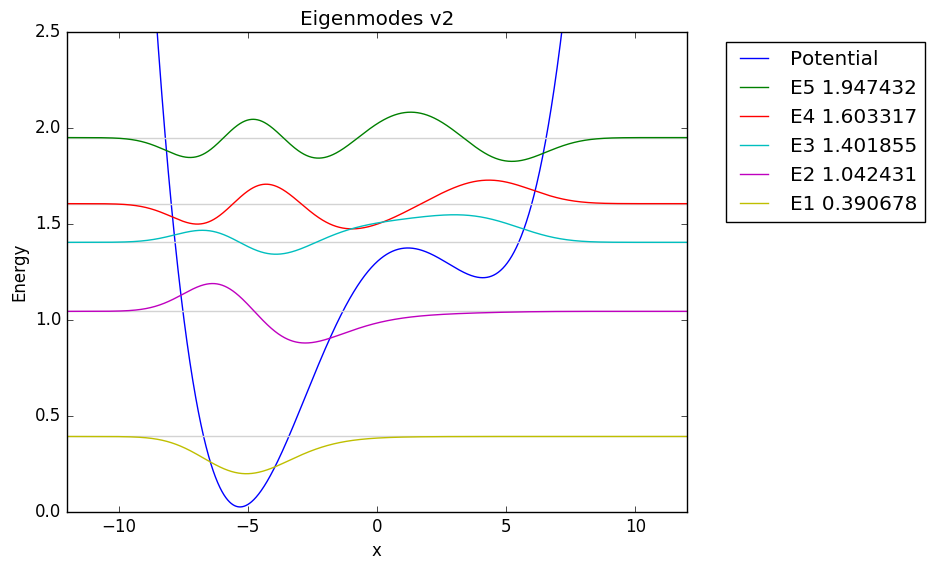
\includegraphics[width=5.5in]{eigv2.png}
\end{figure}

\begin{figure}[h!]
  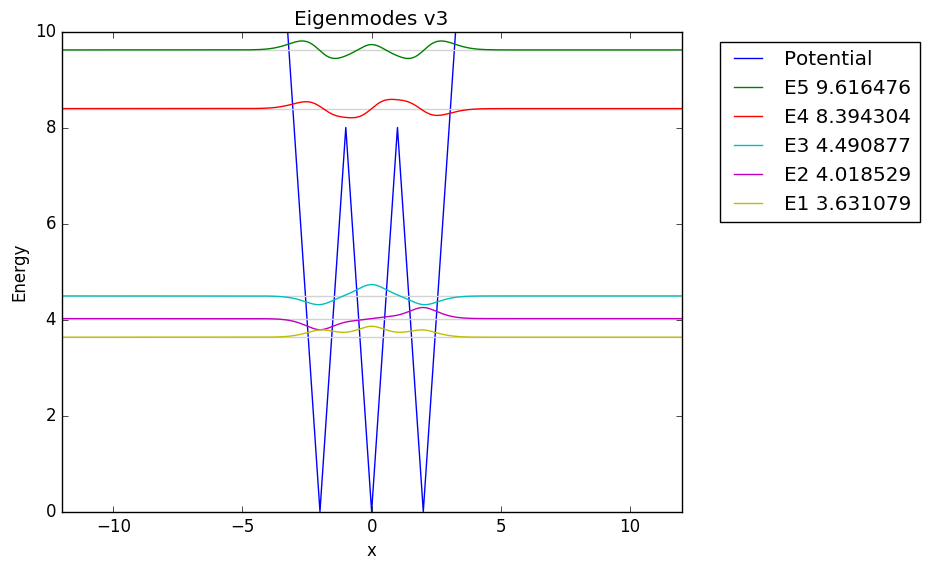
\includegraphics[width=5.5in]{eigv3.png}
\end{figure}

\problem{(b)}

Probability particle lies between 0 and 6 for $v_2$.
\begin{verbatim}
Energies [ 0.39068  1.04243  1.40185  1.60332  1.94743]
Probability [  3.07578e-04   2.99542e-02   7.86516e-01   3.99204e-01   5.33140e-01]
\end{verbatim}

\end{document}